\documentclass [a4paper,12pt,oneside]{article}\usepackage [paper=a4paper,left=37.5264mm,right=37.5264mm,top=37.5264mm,bottom=37.5264mm]{geometry}\usepackage {graphicx}\usepackage {tabularx}\usepackage {alltt}\usepackage {float}\usepackage [section]{placeins}\usepackage {titling}\setlength {\droptitle }{-4em}\pretitle {\begin {flushright}\bfseries \LARGE }\posttitle {\end {flushright}}\preauthor {\begin {flushright}}\postauthor {\end {flushright}}\predate {\begin {flushright}}\postdate {\end {flushright}}\usepackage [english]{babel}\usepackage [T1]{fontenc}\usepackage [utf8x]{inputenc}\usepackage {stmaryrd}\usepackage {amsfonts}\DeclareUnicodeCharacter {12314}{$\llbracket $}\DeclareUnicodeCharacter {12315}{$\rrbracket $}\DeclareUnicodeCharacter {9655}{$\rhd $}\newcommand \nobreakdash {\mbox {-}}\DeclareUnicodeCharacter {8209}{\nobreakdash }\usepackage [sc]{mathpazo}\linespread {1.05}\usepackage [font={small},labelformat=empty,labelsep=none]{caption}\tolerance=10000 \clubpenalty=10000 \widowpenalty=10000 \frenchspacing 

\begin {document}\pagenumbering {roman}\title {Exploring distributed designs with Erlangen: Kademlia}\author {Max Rottenkolber <max@mr.gy>}\date {Thursday, 25 May 2017}\maketitle \pagenumbering {arabic}\setcounter {page}{1}

Common Lisp is known to lend itself to rapid prototyping, and \textit {Erlangen} (\textsf {https:/\allowbreak /\allowbreak github.com/\allowbreak eugeneia/\allowbreak erlangen}) intends to extend these capabilities towards the domain of distributed systems. This article documents an exploration of \textit {distributed hash tables} (\textsf {https:/\allowbreak /\allowbreak en.wikipedia.org/\allowbreak wiki/\allowbreak Distributed\_hash\_table}), specifically the \textit {Kademlia} (\textsf {http:/\allowbreak /\allowbreak www.scs.stanford.edu/\allowbreak {\textasciitilde}dm/\allowbreak home/\allowbreak papers/\allowbreak kpos.pdf}) paper, using Erlangen.

\begin {figure}[H]\centering \includegraphics [width=\columnwidth ]{erlangen-explore-kademlia-dht-big.pdf}\end {figure}

In an attempt to “boldly go where no one has gone before” (not me at least), I present \textit {mesh-table} (\textsf {https:/\allowbreak /\allowbreak github.com/\allowbreak eugeneia/\allowbreak erlangen/\allowbreak blob/\allowbreak mesh-table/\allowbreak platform/\allowbreak mesh-table.lisp}), a distributed hash table design that retains the topology based on the XOR metric pioneered by Kademlia, but otherwise deviates in its goals and implementation. While Kademlia describes a homogeneous peer-to-peer overlay network for exchange of transient data between peers in an untrusted network, mesh-table aims to facilitate storage and retrieval of long-lived, immutable data in a network of dedicated storage and client nodes in a trusted network.

I cover what I perceive to be the core principles of the Kademlia paper (the XOR metric and \textit {k}-buckets), but go astray otherwise, often for simplicity's sake. Don’t expect particularly good ideas that are my own, and by no means production quality code. I’ll just be toying around for fun and insight.

\section* {Distance metric}\addcontentsline {toc}{section}{Distance metric}

Kademlia requires that nodes are assigned identifiers of the same size as the keys used to identify stored values, and relies on the notion of \textit {distance} between two identifiers. The basic premise is that the value denoted by a key is stored on the node with the identifier closest to the key. The distance between two identifiers is defined as their bit-wise XOR.

\begin {figure}[H]\centering \begin {alltt}
(defun distance (x y)
  (logxor x y))
\end{alltt}\vspace {-1em}\end {figure}

\medskip 

\noindent The \texttt {distance} function has some useful properties as a metric of topology. The distance between an identifier and itself is zero

\medskip \medskip 

\noindent \texttt {(distance} \textit {x} \textit {x}\texttt {)} = 0

\medskip \medskip 

\noindent and the distance between two distinct identifiers is positive:

\medskip \medskip 

\noindent \texttt {(distance} \textit {x} \textit {y}\texttt {)} > 0 if \textit {x} ≠ \textit {y}

\medskip \medskip 

\noindent Furthermore, the \texttt {distance} function is symmetric

\medskip \medskip 

\noindent ∀ \textit {x}, \textit {y} : \texttt {(distance} \textit {x} \textit {y}\texttt {)} = \texttt {(distance} \textit {y} \textit {x}\texttt {)}

\medskip \medskip 

\noindent and unidirectional, meaning for any identifier there exists exactly one identifier at any distance:

\medskip \medskip 

\noindent ∀ \textit {x}, \textit {y}, \textit {z} : \texttt {(distance} \textit {x} \textit {y}\texttt {)} ≠ \texttt {(distance} \textit {x} \textit {z}\texttt {)} if \textit {x} ≠ \textit {y} ≠ \textit {z}

\medskip You can imagine the distance metric as a circular railway with each identifier being a train stop, and trains traveling in only one direction. Using the \texttt {distance} function, a node can tell if another node is closer to or further away from a given key, and determine which node is responsible for the key.

\begin {figure}[H]\centering 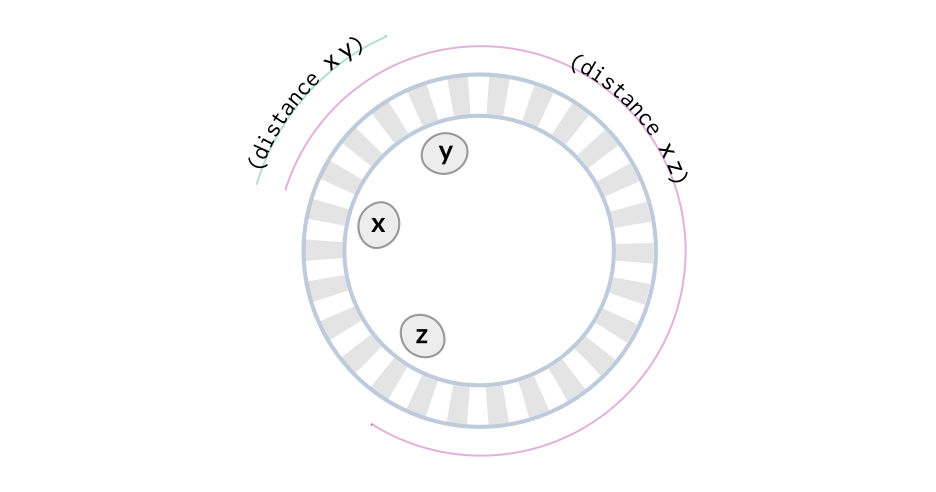
\includegraphics [width=\columnwidth ]{erlangen-explore-kademlia-dht-railway.pdf}\end {figure}



\section* {Routes and buckets}\addcontentsline {toc}{section}{Routes and buckets}

Each Kademlia node maintains a set of \textit {routes} that contain the identifiers and contact details of other nodes, effectively forming an \textit {overlay network} (\textsf {https:/\allowbreak /\allowbreak en.wikipedia.org/\allowbreak wiki/\allowbreak Overlay\_network}). Since our nodes are implemented as \textit {Erlangen agents} (\textsf {http:/\allowbreak /\allowbreak mr.gy/\allowbreak blog/\allowbreak erlangen-intro.html}), we don’t need to deal with network protocols such as UDP, on which Kademlia is traditionally layered upon. Instead, we can use the message passing functionality provided by Erlangen as the underlying network. Hence, our routes store a reference to an agent as the contact information for another node.

Finally, we want to replace routes to nodes that have become inactive with routes to nodes that have more recently contacted us, and so we keep a timestamp with each route to track when we last heard from the node it points to.

\begin {figure}[H]\centering \begin {alltt}
(defstruct (route (:constructor route (id agent)))
  id agent (ctime (get-internal-real-time)))
\end{alltt}\vspace {-1em}\end {figure}

These routes form the edges of a partial mesh network of nodes. Just like keys are stored in the closest node, the mesh is organized by distance. We strive for a network topology that enables efficient lookup and redundancy.

By comparing the identifier in a route to the identifier of the node we can determine the distance of a route. What does that mean, though? After all, our distance metric is not related to geographic distance, or any other “real” metric. Quite the opposite is true: our metric allows us to create a virtual, spatial space in which we can arrange our nodes.

\begin {figure}[H]\centering 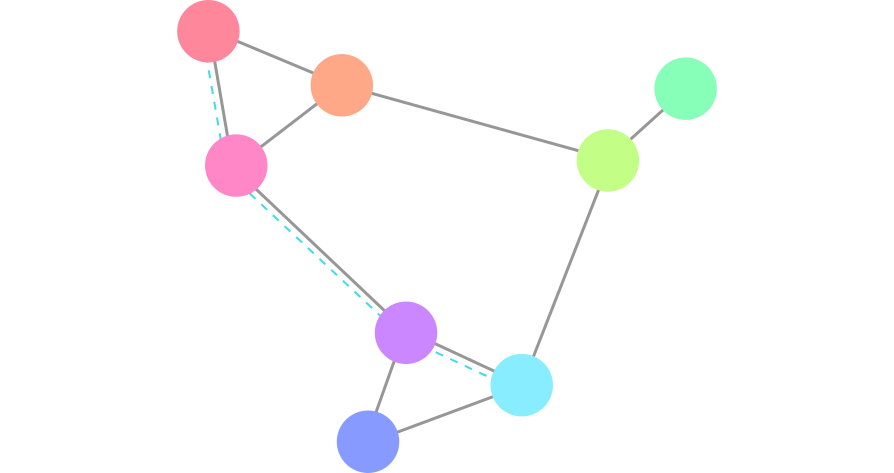
\includegraphics [width=\columnwidth ]{erlangen-explore-kademlia-dht-mesh.pdf}\end {figure}

In this space, nodes keep many routes to nodes close to them, and few routes to distant nodes. If a node receives a request for a given key, and it has a route to a node closer to the key than itself, it forwards the request via the route to the node closest to the key. We can see that a request eventually reaches the closest node in the network, and that the path is optimal with respect to the number of hops.

We implement this by sorting the routes of a node into a fixed number of \textit {buckets}—one for each bit of the identifier—of equally limited capacity, but assign to them exponentially growing ranges of the identifier space. For each 1 ≤ \textit {n} ≤ \textit {keysize}, where \textit {keysize} is the number of bits in an identifier, the respective bucket bucket holds routes to nodes of distance between 2\textit {ⁿ} and 2\textit {ⁿ}⁻¹.

\begin {figure}[H]\centering \includegraphics [width=\columnwidth ]{erlangen-explore-kademlia-dht-buckets.pdf}\end {figure}

A bucket consists of a bound denoting its assigned range (previously \textit {n}), a free-counter to indicate how much capacity is left, and a list of \texttt {*replication*} − \textit {free} routes for 0 ≤ \textit {free} ≤ \texttt {*replication*}. Also, let’s define some of the global constants of our network:

\begin {itemize}\raggedright \item \texttt {*key-size*}—the number of bits that comprise an identifier\item \texttt {*replication*}—a positive integer denoting the replication level of our network (controls the number of routes kept by nodes, as well as how many copies of each stored value we maintain)\end {itemize}

\begin {figure}[H]\centering \begin {alltt}
(defstruct (bucket (:constructor bucket (\&optional (bound *key-size*))))
  bound (free *replication*) routes)

(defun bucket-key-p (bucket distance)
  (< distance (expt 2 (bucket-bound bucket))))

(defun bucket-add (bucket route)
  (push route (bucket-routes bucket))
  (decf (bucket-free bucket)))

(defun bucket-delete (bucket route)
  (setf \#1=(bucket-routes bucket) (delete route \#1\#))
  (incf (bucket-free bucket)))
\end{alltt}\vspace {-1em}\end {figure}

You might notice that \texttt {bucket-key-p} doesn’t implement what I have described, it checks against the upper bound of the bucket range only. That’s because a node starts out with a single bucket initially, and then allocates further buckets on demand. It keeps a list of buckets sorted by increasing bound. The first bucket in that list keeps routes of distance between 0 and 2ⁿ⁻¹, with \textit {n} being the bucket’s bound. Thus, the first bucket contains all routes that don’t fall into any other bucket. To search for a route’s bucket, we can iterate over the bucket list to find the first bucket with an upper bound greater than the distance of the route.

A node also keeps a local mapping from keys to values, as well as a ring of callbacks for outstanding requests, but more on that later.

\begin {figure}[H]\centering \begin {alltt}
(defstruct node
  id (buckets (list (bucket))) values (requests (ring *response-backlog*)))

(defun find-bucket (key node)
  (find-if (let ((distance (distance key (node-id node))))
             (lambda (bucket)
               (bucket-key-p bucket distance)))
           (node-buckets node)))
\end{alltt}\vspace {-1em}\end {figure}

When a new route is to be added to the node’s first bucket and that bucket is full, the next lower bucket is split off the first bucket, and put in front of the bucket list. This allocation strategy makes sense because—depending on the size of our mesh—the lower buckets are increasingly unlikely to be populated, since they hold decreasingly smaller ranges of the identifier space.

\begin {figure}[H]\centering \begin {alltt}
(defun split-bucket (node)
  (let* ((bucket (first (node-buckets node)))
         (new (bucket (1- (bucket-bound bucket)))))
    (dolist (route (bucket-routes bucket))
      (when (bucket-key-p new (distance (route-id route) (node-id node)))
        (bucket-delete bucket route)
        (bucket-add new route)))
    (push new (node-buckets node))))
\end{alltt}\vspace {-1em}\end {figure}

So, when is a bucket full? A bucket is full when its capacity is reached, and none of its routes are \textit {stale}. We consider a route stale once its timestamp exceeds a global timeout constant:

\begin {itemize}\raggedright \item \texttt {*timeout*}—the duration of route validity after the last contact with the route’s node\end {itemize}

\begin {figure}[H]\centering \begin {alltt}
(defun route-stale-p (route)
  (> (- (get-internal-real-time) (route-ctime route))
     *timeout*))

(defun bucket-delete-stale (bucket)
  (let ((stale-route (find-if 'route-stale-p (bucket-routes bucket))))
    (when stale-route
      (bucket-delete bucket stale-route))))
\end{alltt}\vspace {-1em}\end {figure}

With that out of the way, we can formalize how routes are added. First, we find the bucket suitable for the new route, if it has spare capacity, or a stale route can be deleted, we add the route, and are done. If it doesn’t fit, we consider if the bucket in question is the first bucket, in which case it can be split. If it’s not, we simply discard the new route—we’re already well-connected at that distance. Otherwise, we split the first bucket to make room for those close routes, and repeat the process.

\begin {figure}[H]\centering \begin {alltt}
(defun add-route (node route)
  (let ((bucket (find-bucket (route-id route) node)))
    (cond ((or (plusp (bucket-free bucket))
               (bucket-delete-stale bucket))
           (bucket-add bucket route))
          ((eq bucket (first (node-buckets node)))
           (split-bucket node)
           (add-route node route)))))
\end{alltt}\vspace {-1em}\end {figure}

Whenever a node receives a message from another node it already has a route to, it updates that route’s contact information (in case it has changed) and timestamp (preventing it from becoming stale). If the message is from a previously uncontacted node, a new route is added instead. The \texttt {update-route} function below also acts as a predicate that tests whether a matching route exists, and only returns a true when such a route was updated.

\begin {figure}[H]\centering \begin {alltt}
(defun update-route (node id agent)
  (find-if (lambda (route)
             (when (= (route-id route) id)
               (setf (route-agent route) agent
                     (route-ctime route) (get-internal-real-time))))
           (bucket-routes (find-bucket id node))))
\end{alltt}\vspace {-1em}\end {figure}

Finally, we need to be able to find routes to nodes closest to a given identifier. To that end, we sort our routes by distance to said identifier—in descending order because we will select the \textit {n} best routes using \textit {last} (\textsf {http:/\allowbreak /\allowbreak mr.gy/\allowbreak ansi-common-lisp/\allowbreak last.html}). I know, horribly inefficient, but it’s a simple and correct implementation, and that’s all we need right now.

\begin {figure}[H]\centering \begin {alltt}
(defun find-routes (key node)
  (sort (loop for bucket in (node-buckets node)
           append (bucket-routes bucket))
        '> :key (lambda (route)
                  (distance (route-id route) key))))
\end{alltt}\vspace {-1em}\end {figure}



\section* {Callback rings}\addcontentsline {toc}{section}{Callback rings}

We previously defined a node to have a “ring” of callbacks, what’s that about? During their lifetime, nodes send requests to other nodes, and when they do, they include a unique sequence number with each request. When a node responds to a request, it includes the request’s sequence number in its reply. Via the sequence number, the requesting node can then associate the reply with one of its previous requests.

While most of our protocol is stateless, some parts of it do require us to keep track. A node’s requests ring consists of a sequence counter, as well as a buffer of callbacks for a fixed number of requests.

\begin {itemize}\raggedright \item \texttt {*response-backlog*}—the number of callbacks for outstanding requests we keep track of\end {itemize}

The requests ring is implemented as a ring-buffer of virtually unlimited capacity, that overwrites old elements when it wraps around its actual size, and its access function makes sure to return \texttt {nil} instead of the elements that have been overwritten.

\begin {figure}[H]\centering \begin {alltt}
(defstruct ring
  (sequence 0) buffer)

(defun ring (size)
  (make-ring :buffer (make-array size :initial-element nil)))

(defun ring-position (ring sequence)
  (mod sequence (length (ring-buffer ring))))

(defun ring-push (ring value)
  (prog1 \#1=(ring-sequence ring)
    (setf (aref (ring-buffer ring) (ring-position ring \#1\#)) value)
    (incf \#1\#)))

(defun exceeds-ring-p (ring sequence)
  (> (- (ring-sequence ring) sequence) (length (ring-buffer ring))))

(defun ring-get (ring sequence)
  (unless (exceeds-ring-p ring sequence)
    (aref (ring-buffer ring) (ring-position ring sequence))))

(defun ring-delete (ring sequence)
  (unless (exceeds-ring-p ring sequence)
    (setf (aref (ring-buffer ring) (ring-position ring sequence)) nil)))
\end{alltt}\vspace {-1em}\end {figure}

The \texttt {ring} data structure has some very desirable properties, as well as a few questionable trade-offs. The callback ring is of fixed size, thus we avoid the risk of overflow due to excessive outstanding requests. Additionally, we forgo complicated timeout handling, the timeout for outstanding requests is implicitly adjusted relative to the load of the system. The node discards a callback (effectively a timeout of the request) only when it needs to reclaim its buffer slot for a new request. Hence, the effective timeout duration of requests decreases with the request throughput of a node (high load).

\begin {figure}[H]\centering \includegraphics [width=\columnwidth ]{erlangen-explore-kademlia-dht-callback-ring.pdf}\end {figure}

One glaring trade-off is the node’s implied behavior on excessive load. When requests are issued so quickly in succession that the callback ring wraps around before a responding node can reply, the ensuing responses are ignored, causing no progress to be made. Thus, it is up to the client to detect backpressure, and throttle accordingly.

Also noteworthy is how this scheme affects the generational garbage collector. On a system with low load, callbacks can be retained much longer than technically required, possibly causing them to be \textit {tenured} (\textsf {http:/\allowbreak /\allowbreak ccl.clozure.com/\allowbreak docs/\allowbreak ccl.html\#\allowbreak ephemeral-gc}) into an old generation. While this increases GC pressure, I project that this phenomenon is actually amortized, since it is unlikely to occur on medium to high loads—where the additional pressure would actually hurt us.

Importantly, the value of \texttt {*response-backlog*} must be chosen deliberately with these properties in mind, as it governs both the effective timeout duration as well as the peak congestion of the system.



\section* {Protocol messages}\addcontentsline {toc}{section}{Protocol messages}

Our nodes communicate by exchanging and routing messages through the mesh. Usually, this would be the time when we define a wire encoding, but Erlangen does that for us already, so we can simply define structure classes to represent our messages. Each message contains some metadata to facilitate routing, namely the senders node and agent identifiers, in addition to the parameters specific to a particular message type.

\begin {itemize}\raggedright \item \texttt {*node*}—special variable bound to the node’s state, a \texttt {node} structure\end {itemize}

Furthermore, messages are divided into requests and replies. Using \textit {defstruct} (\textsf {http:/\allowbreak /\allowbreak mr.gy/\allowbreak ansi-common-lisp/\allowbreak defstruct.html})’s \texttt {:include} option—which amounts to single-inheritance—we define our different types of messages in a type hierarchy. All types of requests and replies are of type \texttt {message}, but the types \texttt {request} and \texttt {reply} are disjoint.

\begin {figure}[H]\centering 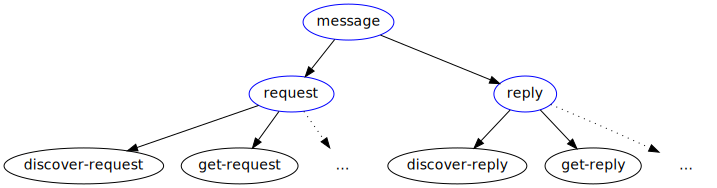
\includegraphics [width=\columnwidth ]{erlangen-explore-kademlia-dht-messages.pdf}\end {figure}

Requests are treated specially because they are subject to being forwarded to the next closer node. They feature two extra flags: \textit {forward-p} and \textit {trace-p}. The former is used for explicit replication by inhibiting forwarding, effectively preventing the receiver from delegating the request. The latter is a debugging feature that allows us to trace how requests travel through the mesh. Replies to requests are always sent directly to the node that originally issued it.

\begin {figure}[H]\centering \begin {alltt}
(defstruct message
  (id (and *node* (node-id *node*))) (agent (agent)) sequence)

(defstruct (request (:include message))
  (forward-p t) trace-p)

(defstruct (reply (:include message)))
\end{alltt}\vspace {-1em}\end {figure}

The semantics for each type of request are expressed as a \texttt {handle} method on the respective type. As mentioned before, nodes shall update or add routes to nodes they are contacted by. To implement this we use CLOS method combination to add a \texttt {:before} method to \texttt {handle} that does just this. Note that since this method is specified on the type \texttt {message}, it is also run when we handle replies.

The body of the method is straight forward, we update the route to the requesting node unless it doesn’t already exist, in which case we add a new route. There is one peculiarity though: some messages won’t have a node identifier, namely the ones issued by client nodes that don’t want to become part of the storage mesh. Client nodes send anonymous requests, and are not interned into the routing tables of other nodes.

\begin {figure}[H]\centering \begin {alltt}
(defmethod handle :before ((message message))
  (with-slots (id agent) message
    (when id
      (or (update-route *node* id agent)
          (add-route *node* (route id agent))))))
\end{alltt}\vspace {-1em}\end {figure}

To help nodes deal with replies we define a function \texttt {reply-bind} that assigns a unique sequence number to a request to be issued, and optionally stores a function in the node’s callback ring under that sequence number. The callback function can then call \texttt {finalize-request} to delete itself, signaling that the request is completed, and preventing further replies to the same request from being accepted. Finally we define a \texttt {handle} method on the \texttt {reply} type to call a respective callback function if applicable.

\begin {figure}[H]\centering \begin {alltt}
(defun reply-bind (request \&optional callback-function)
  (setf (message-sequence request)
        (ring-push (node-requests *node*) callback-function))
  request)

(defun finalize-request (reply)
  (ring-delete (node-requests *node*) (message-sequence reply)))

(defmethod handle ((reply reply))
  (let ((callback (when \#1=(message-sequence reply)
                    (ring-get (node-requests *node*) \#1\#))))
    (when callback
      (funcall callback reply))))
\end{alltt}\vspace {-1em}\end {figure}

Before a request is answered with a reply, it is usually routed forward through the mesh until it arrives at the node responsible for it. Forwarding also plays a role in replication, when a request is forwarded to a set of neighbors to solicit redundancy. For that purpose we define a function \texttt {forward} that sends a request via a list of routes, logging the event when a trace is requested.

\begin {figure}[H]\centering \begin {alltt}
(defun forward (request routes)
  (dolist (route routes routes)
    (when (request-trace-p request)
      (write-log `(:forward ,request ,route)))
    (send request (route-agent route))))
\end{alltt}\vspace {-1em}\end {figure}

When a request has reached its final destination, the respective node responds with a message of type \texttt {reply}, which includes the request’s sequence number. The \texttt {respond} function takes a reply and a request, sets the sequence number of the reply accordingly, and sends it to the agent that initiated the request. When the \textit {trace-p} flag of the request is true the reply is logged.

\begin {figure}[H]\centering \begin {alltt}
(defun respond (reply request)
  (setf (message-sequence reply) (message-sequence request))
  (when (request-trace-p request)
    (write-log `(:respond ,request ,reply)))
  (send reply (message-agent request)))
\end{alltt}\vspace {-1em}\end {figure}

We also define a function \texttt {replicate-request} that creates a copy (or replica) of an request, but overwrites its metadata. It also accepts two optional parameters: \textit {id} and \textit {forward-p}. The \textit {id} parameter sets the node identifier slot of the created replica, and defaults to the calling node’s identifier. Client nodes use this parameter to create anonymous requests by supplying \texttt {nil}. The \textit {forward-p} parameter sets the \textit {forward-p} flag in the replicated request, and defaults to \textit {true}. Its used by storage nodes to explicitly solicit replication, and when they do so they ensure the redundant request isn’t routed by supplying \texttt {nil}.

\begin {figure}[H]\centering \begin {alltt}
(defun replicate-request (request \&key (id (node-id *node*)) (forward-p t))
  (let ((replica (copy-structure request)))
    (setf (message-id replica) id
          (message-agent replica) (agent)
          (message-sequence replica) nil
          (request-forward-p replica) forward-p)
    replica))
\end{alltt}\vspace {-1em}\end {figure}

Finally, we define structures for our set of protocol messages. These are going to be instantiated, as opposed to the previous abstract structure types. Each is a subtype of either \texttt {request} or \texttt {reply}, and may contain one ore more additional slots based on the message’s semantics. These messages include request/reply pairs for discovering new nodes as well as retrieving, storing, and deleting key/value pairs from the mesh.

\begin {figure}[H]\centering \begin {alltt}
(defstruct (discover-request (:include request)) key)
(defstruct (discover-reply (:include reply)))
\end{alltt}\vspace {-1em}\end {figure}

A request of type \texttt {discover-request} includes an extra slot \textit {key} which holds an identifier close to the nodes to be discovered. It is responded to with a reply of type \texttt {discover-reply}, which has no additional slots (the desired information, namely the identifier and agent of the replying node, is already inherited from the \texttt {message} type).

\begin {figure}[H]\centering \begin {alltt}
(defstruct (get-request (:include request)) key)
(defstruct (get-reply (:include reply)) value)
\end{alltt}\vspace {-1em}\end {figure}

A request of type \texttt {get-request} includes an extra slot \textit {key} which holds an identifier used as the key of a value to be retrieved. It is responded to with a reply of type \texttt {get-reply}, which includes an extra slot \textit {value} that holds the value associated with the specified key.

\begin {figure}[H]\centering \begin {alltt}
(defstruct (put-request (:include request)) key value)
(defstruct (put-reply (:include reply)))
\end{alltt}\vspace {-1em}\end {figure}

A request of type \texttt {put-request} includes two extra slots \textit {key} and \textit {value}, which holds an identifier used as a key and a value to be associated with that key. It is responded to with a reply of type \texttt {put-reply}, which merely signifies acknowledgment of the request, and thus has no additional slots.

\begin {figure}[H]\centering \begin {alltt}
(defstruct (delete-request (:include request)) key)
(defstruct (delete-reply (:include reply)))
\end{alltt}\vspace {-1em}\end {figure}

Finally, a request of type \texttt {delete-request} includes an extra slot \textit {key}, which holds an identifier used as a key associated with the value to be deleted. It is responded to with a reply of type \texttt {delete-reply}, which merely signifies acknowledgment of the request, and thus has no additional slots.



\section* {Pluggable stores}\addcontentsline {toc}{section}{Pluggable stores}

By default, we use Common Lisp’s built-in \textit {hash tables} (\textsf {http:/\allowbreak /\allowbreak mr.gy/\allowbreak ansi-common-lisp/\allowbreak Hash-Tables.html\#\allowbreak Hash-Tables}) to store key/value pairs in nodes. This suffices for initial testing and experimentation, but eventually we want to use a persistent storage backend. To that end, we wrap our hash table accesses in methods, implicitly defining a set of generic functions that represents an abstract storage interface.

\begin {figure}[H]\centering \begin {alltt}
(defmethod values-get ((values hash-table) key)
  (gethash key values))

(defmethod values-put ((values hash-table) key value)
  (setf (gethash key values) value))

(defmethod values-delete ((values hash-table) key)
  (remhash key values))
\end{alltt}\vspace {-1em}\end {figure}

By implementing methods for the generic functions \texttt {values-get}, \texttt {values-put}, and \texttt {values-delete} that specialize on the \textit {values} parameter (the store object), we can plug-in alternative storage back-ends later on.



\section* {Protocol logic}\addcontentsline {toc}{section}{Protocol logic}

A central operation during routing is for one node to determine the next hop, if any, for a given request. We define a function \texttt {routes} to be called by a node to find any routes to nodes closer to a given identifier than itself. It accepts a node identifier of the node that initiated the request, and the target identifier of the request (which might be an identifier associated with a value or node), and returns no more than a specified number of relevant routes. By default, up to one route is returned, which will be the best route, if any.

It uses \texttt {find-routes} to get a list of all of the calling node’s routes sorted by distance to the target identifier, and removes from that list all routes that either lead to the node from which the request originated (to prevent routing cycles), are stale, or lead to nodes farther away from the target identifier than the calling node itself. When the calling node has no routes to closer nodes (meaning that its the closest node), \texttt {routes} returns \texttt {nil}.

\begin {figure}[H]\centering \begin {alltt}
(defun routes (from to \&key (limit 1))
  (let ((own-distance (distance (node-id *node*) to)))
    (last (delete-if (lambda (route)
                       (or (eql (route-id route) from)
                           (route-stale-p route)
                           (<= own-distance (distance (route-id route) to))))
                     (find-routes to *node*))
          limit)))
\end{alltt}\vspace {-1em}\end {figure}

A similar function \texttt {neighbors} takes a target identifier, and returns \textit {n} routes closest to the identifier, where \textit {n} defaults to \texttt {*replication*}. An optional boolean parameter controls whether stale routes are excluded.

\begin {figure}[H]\centering \begin {alltt}
(defun neighbors (key \&key include-stale-p (limit *replication*))
  (last (if include-stale-p
            \#1=(find-routes key *node*)
            (delete-if 'route-stale-p \#1\#))
        limit))
\end{alltt}\vspace {-1em}\end {figure}

In order to discover routes to other nodes, and to optionally announce their own existence, nodes send messages of type \texttt {discover-request}. The \texttt {discover} function sends a discover request to its neighbors closest to the identifier \textit {key}. It includes stale routes to eventually reestablish connectivity between temporarily partitioned nodes. The request includes the origin’s identity when \textit {announce-p} is true, effectively announcing its existence to the receiving nodes.

\begin {figure}[H]\centering \begin {alltt}
(defun discover (key \&optional announce-p)
  (forward (if announce-p
               (make-discover-request :key key)
               (make-discover-request :key key :id nil))
           (neighbors key :include-stale-p t)))
\end{alltt}\vspace {-1em}\end {figure}

A node receiving a discover request responds with a message including its identity of type \texttt {discover-reply}, thereby acknowledging its existence. It then forwards the request via up to \texttt {*replication*} routes to nodes closer to the requests \textit {key} identifier.

\begin {figure}[H]\centering \begin {alltt}
(defmethod handle ((request discover-request))
  (with-slots (id key) request
    (respond (make-discover-reply) request)
    (forward request (routes id key :limit *replication*))))
\end{alltt}\vspace {-1em}\end {figure}

Discover requests are redundantly routed through the mesh until they reach the node closest to its target. In the process, the request initiator discovers routes to the closest node and any node along the path. Storage nodes also announce themselves via discover requests, inserting themselves into the mesh by adding or updating routes to themselves. The level of redundancy is controlled by the global \texttt {*replication*} parameter.

\begin {figure}[H]\centering 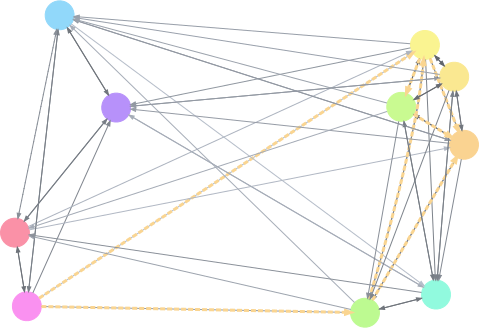
\includegraphics [width=\columnwidth ]{erlangen-explore-kademlia-dht-discover.pdf}\caption {Discover request routed through a mesh of ten nodes with \texttt {*replication*} = 2 (dotted lines represent stale routes).}\end {figure}

The structure of the mesh (see “Routes and buckets”) implies that the paths taken by discover requests are likely to be the shortest possible in terms of the routes available to all nodes, and the number of hops needed to reach a destination does not increase significantly with the size of the identifier space or the size of the network.

To retrieve the value associated with an identifier, nodes send messages of type \texttt {get-request}. The handling node forwards the request to the node closest to the requested key it knows about unless it has no such route (meaning its the closest node), or forwarding is explicitly forbidden (i.e. the \textit {forward-p} flag is false). Once a node is unable to forward a get request, it attempts to retrieve the requested value, and it it exists responds to the initiating node with a message of type \texttt {get-reply}.

If a node can’t satisfy the request because it doesn’t have the requested value, and \textit {forward-p} is true, it replicates the request, sets its \textit {forward-p} flag to false, and forwards it to its neighbors closest to the value’s key. When any of the neighbors replies with the value, the node copies it into its own store before replying to the original request with the retrieved value.

\begin {figure}[H]\centering \begin {alltt}
(defmethod handle ((request get-request))
  (with-slots (id key forward-p) request
    (unless (and forward-p (forward request (routes id key)))
      (multiple-value-bind (value exists-p)
          (values-get \#1=(node-values *node*) key)
        (cond (exists-p
               (respond \#2=(make-get-reply :value value) request))
              (forward-p
               (forward (reply-bind (replicate-request request :forward-p nil)
                                    (lambda (reply)
                                      (with-slots (value) reply
                                        (values-put \#1\# key value)
                                        (respond \#2\# request))
                                      (finalize-request reply)))
                        (neighbors key))))))))
\end{alltt}\vspace {-1em}\end {figure}

The last phase represents somewhat of a failover. If a node can’t satisfy a get request, which it presumably should be able to handle, it calls out to its peers for help as a last resort. Since it will copy any value retrieved this way into its own store, this behavior has a regenerating effect. When a new node joins the mesh, for instance, its store might be empty, but it will receive the subset of get requests closest to its identifier. By calling out to the closest neighbors, of which one must have been responsible for the key before the new node entered the mesh, it will over time accumulate all the values its responsible for.

\begin {figure}[H]\centering 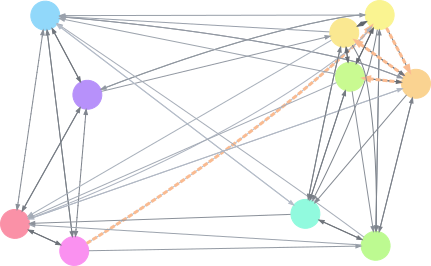
\includegraphics [width=\columnwidth ]{erlangen-explore-kademlia-dht-get.pdf}\caption {Unsuccessful get request routed through a mesh of ten nodes with \texttt {*replication*} = 2. The request is replicated at the destination because no value associated with the key is present.}\end {figure}

Because of how the mesh is structured, the handling node should be in a good position to coordinate with the next closest nodes. It it more likely than any other node to have routes to any nodes that store values for keys close to its identifier.

In order to store values in the mesh, nodes send messages of type \texttt {put-request} that contain the key identifier and the value to be associated with it. Put requests are forwarded through the mesh just like get requests are. Finally, the handling node records the key/value pair, and additionally replicates the requests to its neighbors closest to the key.

\begin {figure}[H]\centering \begin {alltt}
(defmethod handle ((request put-request))
  (unless (and forward-p (forward request (routes id key)))
    (values-put (node-values *node*) key value)
    (respond (make-put-reply) request)
    (when forward-p
      (forward (replicate-request request :forward-p nil)
               (neighbors key)))))
\end{alltt}\vspace {-1em}\end {figure}

By forwarding copies of the request, the handling node distributes the key/value pair redundantly to the next closer nodes. If all goes well, a successful put requests leaves \textit {n}+1 copies of the pair in the mesh, where \textit {n} = \texttt {*replication*}. Just as with get requests, the handling node’s affinity to other nodes close to the key identifier ensures that it will be able to replicate the value to relevant nodes.

\begin {figure}[H]\centering 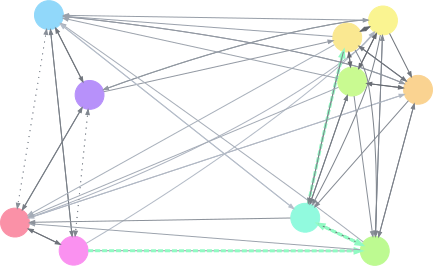
\includegraphics [width=\columnwidth ]{erlangen-explore-kademlia-dht-put.pdf}\caption {Put request routed through a mesh of ten nodes with \texttt {*replication*} = 2. The request is replicated at the destination to store the value redundantly.}\end {figure}

Finally, nodes can delete values associated with a key by issuing messages of type \texttt {delete-request}. It works almost exactly like a put request, except that it removes key/value pairs from a node’s records.

\begin {figure}[H]\centering \begin {alltt}
(defmethod handle ((request delete-request))
  (with-slots (id key forward-p) request
    (unless (and forward-p (forward request (routes id key)))
      (values-delete (node-values *node*) key)
      (respond (make-delete-reply) request)
      (when forward-p
        (forward (replicate-request request :forward-p nil)
                 (neighbors key))))))
\end{alltt}\vspace {-1em}\end {figure}

Since routes become stale over time, a period of low or no traffic might leave a node without fresh routes. To avoid this situation, nodes periodically refresh buckets that are not full or contain stale routes. A bucket is refreshed by performing discover requests on a random identifier that falls within that bucket.

The function \texttt {refresh-routes} performs the procedure outlined above. It accepts a boolean parameter \textit {announce-p} that controls whether the calling node should announce itself to its peers.

The inner workings of \texttt {refresh-routes} are a bit tricky. Remember that the first bucket contains all routes that don’t fall into any other bucket, so the first bucket spans the range of identifiers starting at distance \textit {d} = 1 (the identifier at distance \textit {d} = 0 is the node’s own identifier). For each bucket to refresh, we generate a random distance within its range, and attempt to discover the node with the identifier at that distance.

Remember that our distance function is unidirectional: for any identifier there exists exactly one identifier at any distance. Since our \texttt {distance} function is defined as \texttt {logxor}, the following holds true

\medskip 

\noindent \texttt {(distance} \textit {x} \textit {y}\texttt {)} = \textit {d} → \texttt {(distance} \textit {x} \textit {d}\texttt {)} = \textit {y}

\medskip and we can obtain an identifier within the bucket by computing the distance between the calling node’s identifier and the distance selected at random.

\begin {figure}[H]\centering \begin {alltt}
(defun refresh-routes (\&optional announce-p)
  (loop for bucket in (node-buckets *node*)
        for start = 1 then end
        for end = (expt 2 (bucket-bound bucket))
     do (when (or (plusp (bucket-free bucket))
                  (find-if 'route-stale-p (bucket-routes bucket)))
          (discover (distance (+ start (random (- end start)))
                              (node-id *node*))
           announce-p))))
\end{alltt}\vspace {-1em}\end {figure}

When a node is first started it is supplied a set of initial peers. The function \texttt {initialize-node} takes a list of identifier/agent pairs, and adds a new route for each entry. It then performs discover requests on the node’s own identifier using the initial routes. The optional parameter \textit {announce-p} controls whether the calling node should announce itself to its peers.

\begin {figure}[H]\centering \begin {alltt}
(defun initialize-node (initial-peers \&optional announce-p)
  (loop for (id agent) in initial-peers do
       (add-route *node* (route id agent)))
  (discover (node-id *node*) announce-p))
\end{alltt}\vspace {-1em}\end {figure}

In order to perform periodic actions (like refreshing routes in our case) we need to keep track of time and time intervals. For this we use \texttt {get-internal-real-time}¹ to get a \textit {monotonic time} (\textsf {https:/\allowbreak /\allowbreak www.softwariness.com/\allowbreak articles/\allowbreak monotonic-clocks-windows-and-posix/\allowbreak }). Monotony is important in this context because we care about stable intervals specifically, and want them to be strictly dependent on elapsed time—as opposed to global time. \texttt {Get-internal-real-time} returns a time in “internal time units”, which can be converted to seconds using the constant \texttt {internal-time-units-per-second}.

The function \texttt {deadline} accepts a timeout in internal time units, and returns a deadline (a time in the future at which the timeout will be exceeded). Analogous, the function \texttt {deadline-exceeded-p} is a predicate that accepts a deadline, and tests whether it is exceeded.

The function \texttt {receive-until} accepts a deadline, and waits to receive a message until the deadline is exceeded. It returns either a message received by the calling agent, or signals an error of type \texttt {timeout} if the deadline was exceeded. It uses the function \texttt {seconds-until-deadline} which returns the seconds left until a time in internal time units will pass. \texttt {Receive-until} lets us multitask between handling incoming messages and performing our periodic duties on time by ensuring that we don’t miss a deadline while we wait for incoming messages.

\begin {figure}[H]\centering \begin {alltt}
(defun deadline (timeout)
  (+ (get-internal-real-time) timeout))

(defun deadline-exceeded-p (deadline)
  (>= (get-internal-real-time) deadline))

(defun seconds-until-deadline (deadline)
  (/ (max (- deadline (get-internal-real-time)) 0)
     internal-time-units-per-second))

(defun receive-until (deadline)
  (if (deadline-exceeded-p deadline)
      (error 'timeout))
      (receive :timeout (seconds-until-deadline deadline)))
\end{alltt}\vspace {-1em}\end {figure}

\begin {itemize}\raggedright \item 1. At the time of writing CCL’s \texttt {get-internal-real-time} is undocumented, and even \textit {broken} (\textsf {https:/\allowbreak /\allowbreak github.com/\allowbreak Clozure/\allowbreak ccl/\allowbreak issues/\allowbreak 20}). Erlangen includes a \textit {fixed version} (\textsf {https:/\allowbreak /\allowbreak github.com/\allowbreak eugeneia/\allowbreak erlangen/\allowbreak blob/\allowbreak b3c440d2104883893b82e3372a5447d4f55ca013/\allowbreak ccl.lisp\#\allowbreak L26}) of this function for the meantime, at least for platforms other than MS Windows.\end {itemize}



\section* {Storage nodes and clients}\addcontentsline {toc}{section}{Storage nodes and clients}

Now we have assembled all the pieces needed to express the life cycle of a node. The functions \texttt {node} and \texttt {client}, that implement the behavior of a storage node and a client respectively, are intended to be used as top-level functions for agents (i.e. as the first argument to \textit {spawn} (\textsf {http:/\allowbreak /\allowbreak mr.gy/\allowbreak software/\allowbreak erlangen/\allowbreak api.html\#\allowbreak section-1-14})).

A storage node is initialized with an identifier, a set of initial peers, and a store object that maps keys to values. First, it binds \textit {*random-state*} (\textsf {http:/\allowbreak /\allowbreak mr.gy/\allowbreak ansi-common-lisp/\allowbreak \_002arandom\_002dstate\_002a.html}) to a fresh random state object that has been randomly initialized to get its own independently seeded random source to generate random identifiers. It then binds the special variable \texttt {*node*} to a fresh \texttt {node} structure which is initialized as follows: unless specified, the identifier is selected at random using \texttt {gen-id}, and an empty hash table is used for storing values.

Additionally, an interval at half of the duration of \texttt {*timeout*} is set, to be used as the refresh deadline. The deadline is selected at halfway to the expiry date of fresh routes, so that newly added routes can be pinged at least once before they become stale. The first deadline is set to expire after a random duration up to the interval in order to avoid a \textit {thundering herd} (\textsf {https:/\allowbreak /\allowbreak en.wikipedia.org/\allowbreak wiki/\allowbreak Thundering\_herd\_problem}) situation.

The node then initializes routes to its initial peers, and announces itself before entering its event loop. If a message is received before the refresh deadline expires it is processed according to protocol by \texttt {handle}. When the refresh deadline is met it is reset, and the node’s routes are refreshed.

\begin {figure}[H]\centering \begin {alltt}
(defun gen-id ()
  (random (expt 2 *key-size*)))

(defun node (\&key id initial-peers values)
  (let* ((*random-state* (make-random-state t))
         (*node* (make-node :id (or id (gen-id))
                            :values (or values (make-hash-table))))
         (refresh-interval (/ *timeout* 2))
         (refresh-deadline (deadline (random refresh-interval))))
    (initialize-node initial-peers :announce)
    (loop do (handler-case (handle (receive-until refresh-deadline))
               (timeout (refresh-deadline-exceeded)
                 (declare (ignore refresh-deadline-exceeded))
                 (setf refresh-deadline (deadline refresh-interval))
                 (refresh-routes :announce))))))
\end{alltt}\vspace {-1em}\end {figure}

Clients behave very similar to storage nodes, except they always use a randomly generated identifier, and do not use a store object. A client doesn’t announce itself, and proxies incoming requests instead of handling them. As such, it serves as a gateway into the mesh that can be used by one or more agents.

The function \texttt {proxy} takes a request, and forwards an anonymous replica of the request via its route to the node closest to the request key. It installs a callback to handle the eventual response, which causes the client to respond to the request issuer with the reply.

\begin {figure}[H]\centering \begin {alltt}
(defun proxy (request)
  (forward (reply-bind (replicate-request request :id nil)
                       (lambda (reply)
                         (finalize-request reply)
                         (respond reply request)))
           (neighbors (slot-value request 'key) :limit 1)))

(defun client (\&key initial-peers)
  (let* ((*random-state* (make-random-state t))
         (*node* (make-node :id (gen-id)))
         (refresh-interval (/ *timeout* 2))
         (refresh-deadline (deadline (random refresh-interval))))
    (initialize-node initial-peers)
    (loop do (handler-case (let ((message (receive-until refresh-deadline)))
                             (etypecase message
                               ((cons agent request) (proxy (cdr message)))
                               (reply (handle message))))
               (timeout (refresh-deadline-exceeded)
                 (declare (ignore refresh-deadline-exceeded))
                 (setf refresh-deadline (deadline refresh-interval))
                 (refresh-routes))))))
\end{alltt}\vspace {-1em}\end {figure}

If you are wondering why \texttt {client} accepts messages of the form \texttt {(}\textit {agent} \texttt {.} \textit {request}\texttt {)} even though it never looks at the agent value, and sends replies back to the agent noted in the request structure, wonder no more. This way, clients implement the \texttt {erlangen-plaform.server} protocol, and can be can be queried using \texttt {cast} and \texttt {call}.



\section* {Taking the mesh for a spin}\addcontentsline {toc}{section}{Taking the mesh for a spin}

Let’s go for a test drive. If you want to follow along, make sure to check out the \texttt {mesh-table} branch, and load \texttt {erlangen-platform}. First, we define a fresh package to experiment in, with all the goodies we need.

\begin {figure}[H]\centering \begin {alltt}
(ql:quickload :erlangen-platform)

(defpackage mesh-table-user
  (:use :cl
        :erlangen
        :erlangen-platform.log
        :erlangen-platform.server
        :erlangen-platform.mesh-table)
  (:shadowing-import-from :erlangen-platform.server :call)
  (:shadowing-import-from :erlangen-platform.mesh-table :node))

(in-package :mesh-table-user)
\end{alltt}\vspace {-1em}\end {figure}

To bootstrap the mesh, we generate a random identifier, and use it to spawn our first node—the root node. So far it’s a lone wolf, but at least now we have an initial peer we can use to initialize further nodes with.

\begin {figure}[H]\centering \begin {alltt}
(defparameter *root-id* (gen-id))
(defparameter *root-node* (spawn `(node :id ,*root-id*)))
\end{alltt}\vspace {-1em}\end {figure}

Now we can populate the mesh with a bunch of nodes. Initially, they will only have one peer (the root node), but it won’t be long until they discover each other.

\begin {figure}[H]\centering \begin {alltt}
(defparameter *nodes* ())
(dotimes (i 20)
  (push (spawn `(node :initial-peers ((,*root-id* ,*root-node*))))
        *nodes*))
\end{alltt}\vspace {-1em}\end {figure}

\begin {figure}[H]\centering 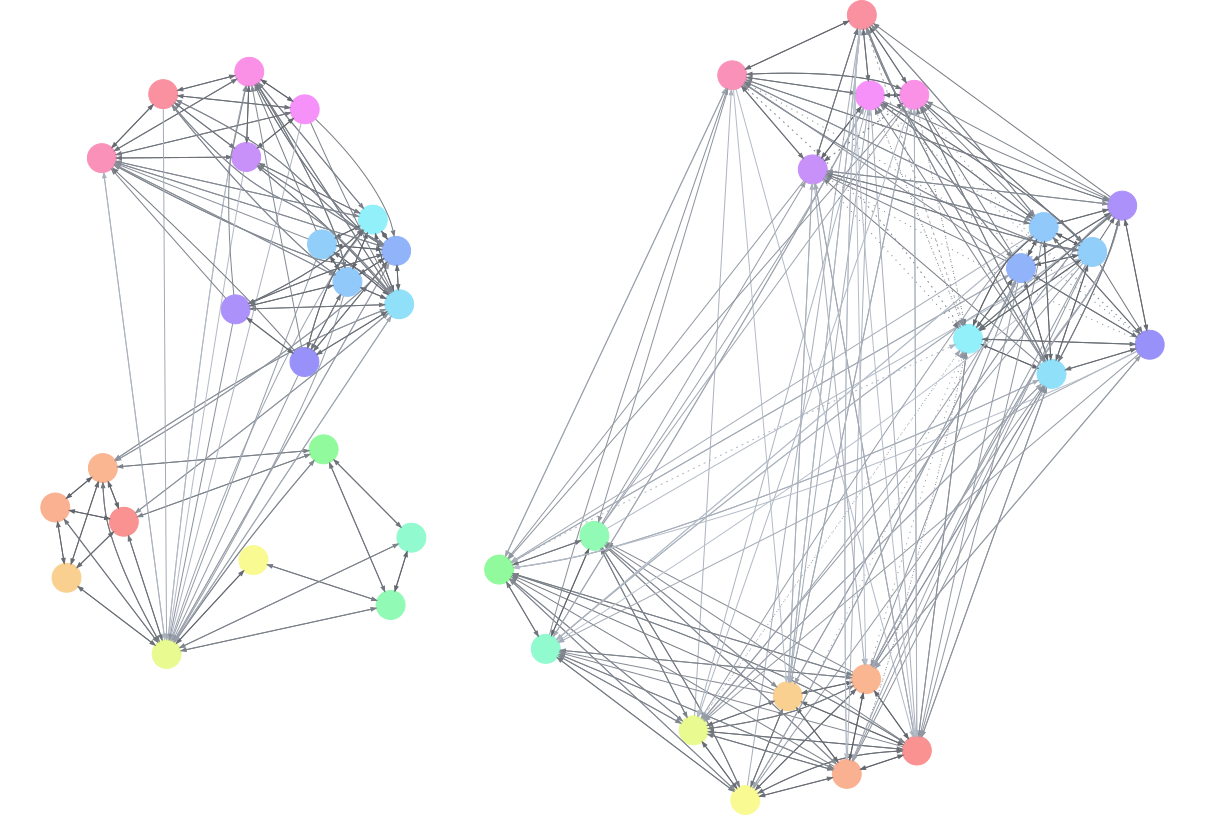
\includegraphics [width=\columnwidth ]{erlangen-explore-kademlia-dht-spin.pdf}\caption {On the left: the mesh right after we spawned the majority of nodes, the root node is clearly discernible. On the right: after a while, nodes discover more relevant routes, and seldom used routes become stale.}\end {figure}

Of course we want to interact with the mesh, so let’s spawn a client node, and put some data into the network. We generate a few random keys, and call the client with put requests to insert some values. Each put request yields a put reply acknowledging the operation.

\begin {figure}[H]\centering \begin {alltt}
(defparameter *client*
  (spawn `(client :initial-peers ((,*root-id* ,*root-node*)))))

(defparameter *keys* (list (gen-id) (gen-id) (gen-id)))

(call *client* (make-put-request :key (first *keys*) :value 1))
→ \#S(ERLANGEN-PLATFORM.MESH-TABLE::PUT-REPLY
     :ID 293999586930477495619460952165128733173
     :AGENT \#<AGENT ERLANGEN-PLATFORM.MESH-TABLE:NODE \#x30200349411D>
     :SEQUENCE NIL)

(call *client* (make-put-request :key (second *keys*) :value 2))
→ …

(call *client* (make-put-request :key (third *keys*) :value 3))
→ …
\end{alltt}\vspace {-1em}\end {figure}

\begin {figure}[H]\centering 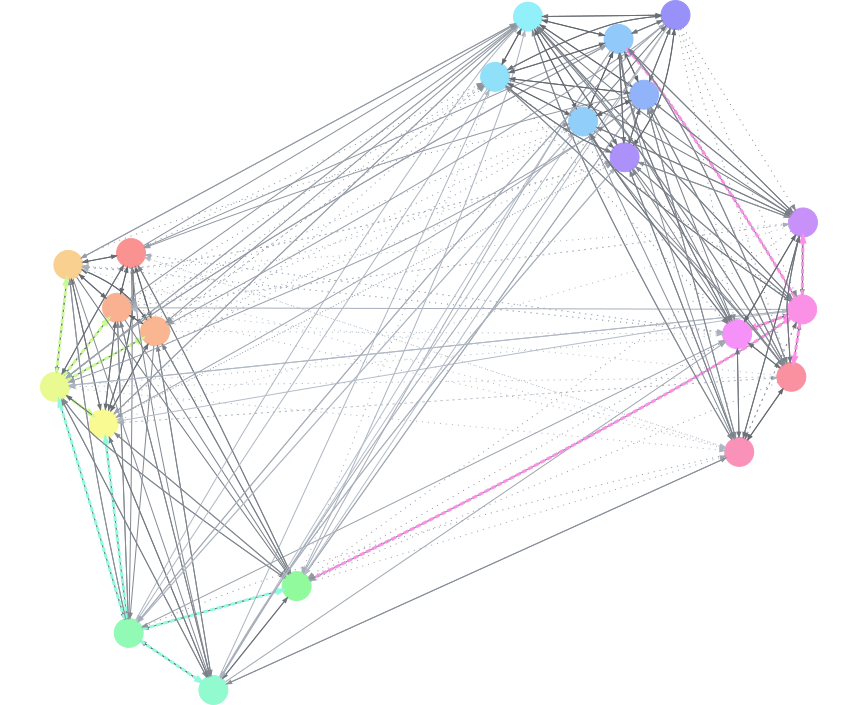
\includegraphics [width=\columnwidth ]{erlangen-explore-kademlia-dht-spin-put.pdf}\caption {Our three put requests routed through the mesh, and stored redundantly.}\end {figure}

To get more insight into what happens behind the scenes, we can trace requests through the mesh. But first, we need to spawn a logging agent to log the trace. We register the name \texttt {:log} for our logger, which is the default destination for \texttt {write-log} (on top of which our tracing is built on).

\begin {figure}[H]\centering \begin {alltt}
(register :log :agent (spawn 'logger))
\end{alltt}\vspace {-1em}\end {figure}

With a log present, we can trace our requests using the \texttt {:trace-p} flag. Let’s trace a get request, and see what happens. The client forwards the request to the node closest to the key. Since the client just handled a put request to the same key, it still has a direct route to the node closest to the key, and that node happens to be final destination for the request. The node responds with a get reply to the client, which then responds to the caller.

\begin {figure}[H]\centering \begin {alltt}
(call *client* (make-get-request :key (first *keys*) :trace-p t))
▷ ("2017-05-24 13:00:57"
▷  \#<AGENT ERLANGEN-PLATFORM.MESH-TABLE:CLIENT \#x3020034FAA5D> :FORWARD
▷  \#S(ERLANGEN-PLATFORM.MESH-TABLE::GET-REQUEST
▷     :ID NIL
▷     :AGENT \#<AGENT ERLANGEN-PLATFORM.MESH-TABLE:CLIENT \#x3020034FAA5D>
▷     :SEQUENCE 3
▷     :FORWARD-P T
▷     :TRACE-P T
▷     :KEY 155130510100689072426815715566014896677)
▷  \#S(ERLANGEN-PLATFORM.MESH-TABLE::ROUTE
▷     :ID 132185931380890600385825626482768187951
▷      :AGENT \#<AGENT ERLANGEN-PLATFORM.MESH-TABLE:NODE \#x30200349EB8D>
▷      :CTIME 1702536187961))
▷ ("2017-05-24 13:00:57"
▷  \#<AGENT ERLANGEN-PLATFORM.MESH-TABLE:NODE \#x30200349EB8D> :RESPOND
▷  \#S(ERLANGEN-PLATFORM.MESH-TABLE::GET-REQUEST
▷     :ID NIL
▷     :AGENT \#<AGENT ERLANGEN-PLATFORM.MESH-TABLE:CLIENT \#x3020034FAA5D>
▷     :SEQUENCE 3
▷     :FORWARD-P T
▷     :TRACE-P T
▷     :KEY 155130510100689072426815715566014896677)
▷  \#S(ERLANGEN-PLATFORM.MESH-TABLE::GET-REPLY
▷     :ID 132185931380890600385825626482768187951
▷     :AGENT \#<AGENT ERLANGEN-PLATFORM.MESH-TABLE:NODE \#x30200349EB8D>
▷     :SEQUENCE NIL
▷     :VALUE 1))
▷ ("2017-05-24 13:00:57"
▷  \#<AGENT ERLANGEN-PLATFORM.MESH-TABLE:CLIENT \#x3020034FAA5D> :RESPOND
▷  \#S(ERLANGEN-PLATFORM.MESH-TABLE::GET-REQUEST
▷     :ID NIL
▷     :AGENT \#<AGENT \#x30200337635D>
▷     :SEQUENCE NIL
▷     :FORWARD-P T
▷     :TRACE-P T
▷     :KEY 155130510100689072426815715566014896677)
▷  \#S(ERLANGEN-PLATFORM.MESH-TABLE::GET-REPLY
▷     :ID 132185931380890600385825626482768187951
▷     :AGENT \#<AGENT ERLANGEN-PLATFORM.MESH-TABLE:NODE \#x30200349EB8D>
▷     :SEQUENCE NIL
▷     :VALUE 1))
→ \#S(ERLANGEN-PLATFORM.MESH-TABLE::GET-REPLY
     :ID 132185931380890600385825626482768187951
     :AGENT \#<AGENT ERLANGEN-PLATFORM.MESH-TABLE:NODE \#x30200349EB8D>
     :SEQUENCE NIL
     :VALUE 1)
\end{alltt}\vspace {-1em}\end {figure}

So far so good, let’s kill half of our nodes to see how the mesh deals with that. Imagine a whole data center burns down to the ground, and no backups can be found. In distributed speak this situation is called a partition, which implies that the nodes could come back up at a later time, but in our case they won’t.

\begin {figure}[H]\centering \begin {alltt}
(dotimes (i 10)
  (exit :kill (pop *nodes*)))
\end{alltt}\vspace {-1em}\end {figure}

\begin {figure}[H]\centering 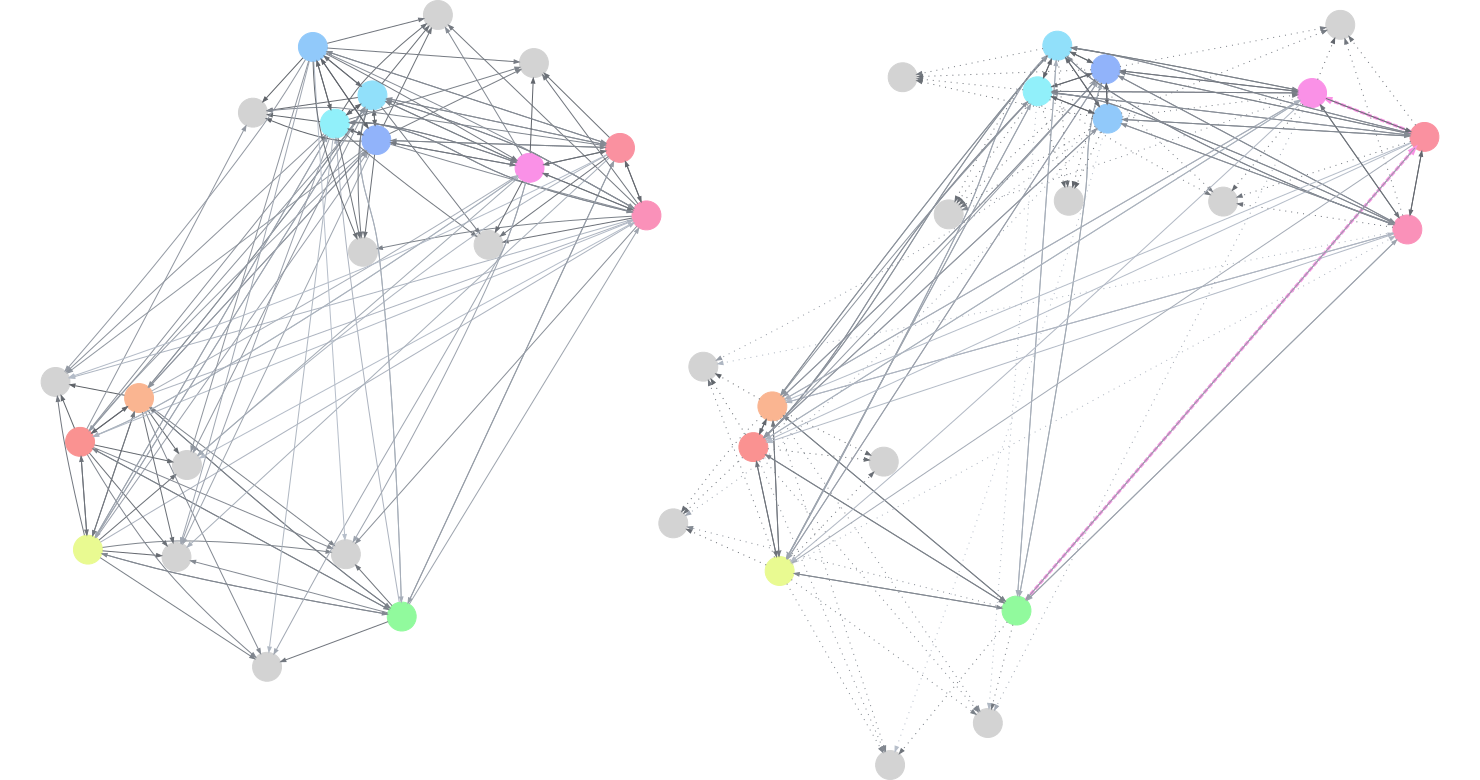
\includegraphics [width=\columnwidth ]{erlangen-explore-kademlia-dht-spin-partition.pdf}\caption {On the left: the mesh right after the disaster. On the right: routes to dead nodes become stale, and the get request finds its way to a redundant node.}\end {figure}

We can still make requests, but we might not get back an reply—half of our mesh went dark after all. We can supply a timeout to \texttt {call} to give an upper bound to the time we wait to a reply. The request might be forwarded through a seemingly fine route, to a node that won’t reply no matter what. After a while though, the routes to dead nodes will become stale. A live node will take over, and chances are high that it will be able to yield the correct value.

\begin {figure}[H]\centering \begin {alltt}
(call *client* (make-get-request :key (first *keys*))
      :timeout 1)
→ \#S(ERLANGEN-PLATFORM.MESH-TABLE::GET-REPLY
     :ID 119982038210290876000818395666614461298
     :AGENT \#<AGENT ERLANGEN-PLATFORM.MESH-TABLE:NODE \#x3020034A570D>
     :SEQUENCE NIL
     :VALUE 1)
\end{alltt}\vspace {-1em}\end {figure}

To make up for our losses, we spawn ten fresh nodes to take over. New routes are established, and some stale are routes forgotten. Soon enough the mesh will look just as healthy as it did before.

\begin {figure}[H]\centering \begin {alltt}
(dotimes (i 10)
  (push (spawn `(node :initial-peers ((,*root-id* ,*root-node*))))
        *nodes*))
\end{alltt}\vspace {-1em}\end {figure}

\begin {figure}[H]\centering 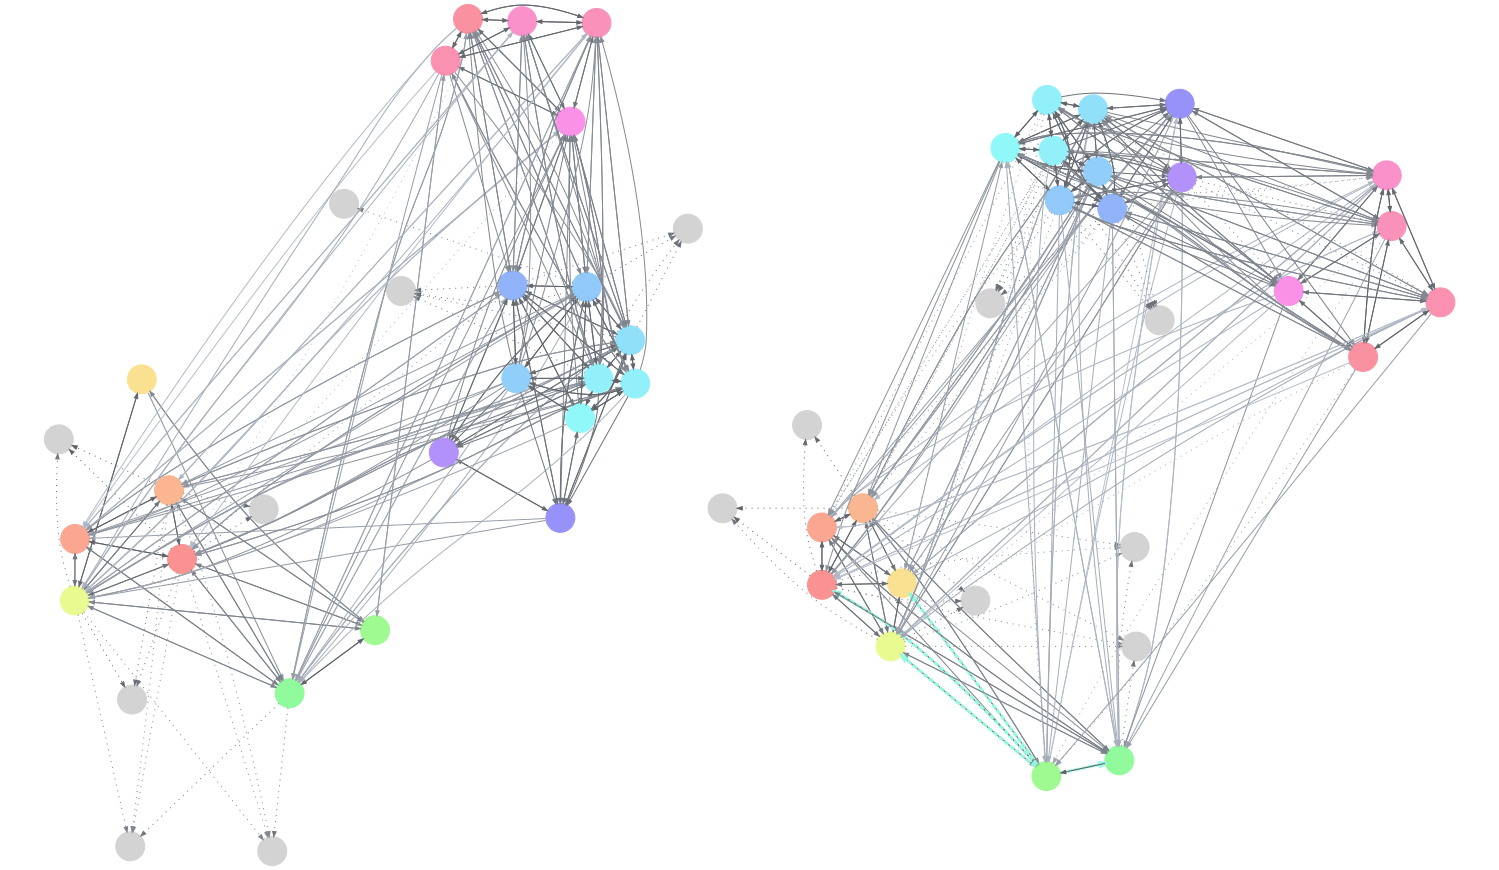
\includegraphics [width=\columnwidth ]{erlangen-explore-kademlia-dht-spin-regenerate.pdf}\caption {On the left: the mesh right after we added the fresh nodes. On the left: a little while later, a new node asks its neighbors for a record it should have.}\end {figure}

Over time, the new nodes will even regenerate records previously owned by now dead nodes. When a node receives a get request for a key to which it is closest, but doesn’t have a value for the key, it forwards the request to its neighbors with the \texttt {forward-p} flag set to \texttt {nil}. If it gets a reply it copies the value into its own store, and replies as if it had always been present.

\begin {figure}[H]\centering \begin {alltt}
(call *client* (make-get-request :key (first *keys*) :trace-p t))
▷ …
▷ ("2017-05-24 13:59:35"
▷  \#<AGENT ERLANGEN-PLATFORM.MESH-TABLE:NODE \#x3020035127FD> :FORWARD
▷  \#S(ERLANGEN-PLATFORM.MESH-TABLE::GET-REQUEST
▷     :ID 106415979122184563321987569594398713625
▷     :AGENT \#<AGENT ERLANGEN-PLATFORM.MESH-TABLE:NODE \#x3020035127FD>
▷     :SEQUENCE 0
▷     :FORWARD-P NIL
▷     :TRACE-P T
▷     :KEY 155130510100689072426815715566014896677)
▷  \#S(ERLANGEN-PLATFORM.MESH-TABLE::ROUTE
▷     :ID 411292742280498946490320458060617158
▷     :AGENT \#<AGENT ERLANGEN-PLATFORM.MESH-TABLE:NODE \#x3020034933AD>
▷     :CTIME 1706058833487))
▷ ("2017-05-24 13:59:35"
▷  \#<AGENT ERLANGEN-PLATFORM.MESH-TABLE:NODE \#x3020035127FD> :FORWARD
▷  \#S(ERLANGEN-PLATFORM.MESH-TABLE::GET-REQUEST
▷     :ID 106415979122184563321987569594398713625
▷     :AGENT \#<AGENT ERLANGEN-PLATFORM.MESH-TABLE:NODE \#x3020035127FD>
▷     :SEQUENCE 0
▷     :FORWARD-P NIL
▷     :TRACE-P T
▷     :KEY 155130510100689072426815715566014896677)
▷  \#S(ERLANGEN-PLATFORM.MESH-TABLE::ROUTE
▷     :ID 43349484706135223247500409734337076500
▷     :AGENT \#<AGENT ERLANGEN-PLATFORM.MESH-TABLE:NODE \#x30200352189D>
▷     :CTIME 1706033691806))
▷ …
▷ ("2017-05-24 13:59:35"
▷  \#<AGENT ERLANGEN-PLATFORM.MESH-TABLE:NODE \#x3020034A570D> :RESPOND
▷  \#S(ERLANGEN-PLATFORM.MESH-TABLE::GET-REQUEST
▷     :ID 106415979122184563321987569594398713625
▷     :AGENT \#<AGENT ERLANGEN-PLATFORM.MESH-TABLE:NODE \#x3020035127FD>
▷     :SEQUENCE 0
▷     :FORWARD-P NIL
▷     :TRACE-P T
▷     :KEY 155130510100689072426815715566014896677)
▷  \#S(ERLANGEN-PLATFORM.MESH-TABLE::GET-REPLY
▷     :ID 119982038210290876000818395666614461298
▷     :AGENT \#<AGENT ERLANGEN-PLATFORM.MESH-TABLE:NODE \#x3020034A570D>
▷     :SEQUENCE 0
▷     :VALUE 1))
▷ …
→ \#S(ERLANGEN-PLATFORM.MESH-TABLE::GET-REPLY
     :ID 106415979122184563321987569594398713625
     :AGENT \#<AGENT ERLANGEN-PLATFORM.MESH-TABLE:NODE \#x3020035127FD>
     :SEQUENCE NIL
     :VALUE 1)
\end{alltt}\vspace {-1em}\end {figure}

That’s it for out little tour through the mesh. I hope I could show some weaknesses (like reduced availability right after partition), and some strengths (like effective durability) of the design. Most importantly, I hope I could convince you of Common Lisp and Erlangen as a good platform for developing distributed designs.



\section* {Appendix: graphing the mesh}\addcontentsline {toc}{section}{Appendix: graphing the mesh}

You might have guessed that the visual graphs of meshes found in this article were not created by hand. The \texttt {mesh-table} branch comes with some \textit {extra code} (\textsf {https:/\allowbreak /\allowbreak github.com/\allowbreak eugeneia/\allowbreak erlangen/\allowbreak blob/\allowbreak mesh-table/\allowbreak platform/\allowbreak mesh-table-graphviz.lisp}) for rendering live mesh networks using \textit {Graphviz} (\textsf {http:/\allowbreak /\allowbreak graphviz.org/\allowbreak }), specifically a \textit {DOT} (\textsf {https:/\allowbreak /\allowbreak en.wikipedia.org/\allowbreak wiki/\allowbreak DOT\_\%28graph\_description\_language\%29}) emitter.

Identifiers are encoded in the color space, which can sometimes be misleading, but gives a fairly accurate sense of distance most of the time. Edge length and thickness also relate to the distance between two nodes connected by a route. Additionally, it adds visual cues for stale routes, dead nodes, and can even overlay request traces onto the graph.

Besides generating visual graphs for this article, the DOT emitter also proved to be an invaluable debugging tool. Bugs that might otherwise be subtle, become very prominent, if not obvious, when you can see them affect the live system. In fact, as the visualization improved, I found more and more bugs. I can’t stress enough, how (even more) embarrassingly bug ridden this article would’ve been, if the little \texttt {graphviz} function hadn’t saved the day.



\end {document}